{
\renewcommand{\baselinestretch}{1.0}
\begin{figure}[t]
\begin{center}
\subfigure[Scaling a PDS sort benchmark up to 25 nodes.]{
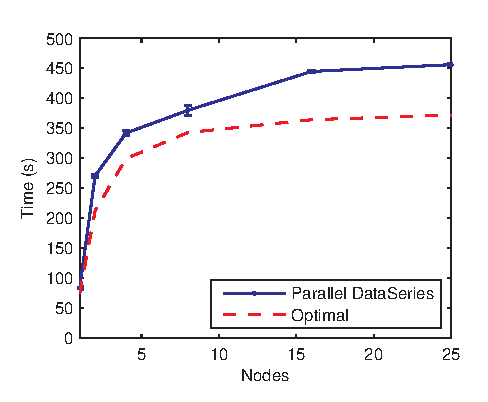
\includegraphics{fig_pds_sort2.eps}
\label{fig:pds:sort2:scale}
}
\subfigure[Time breakdown into phases.]{
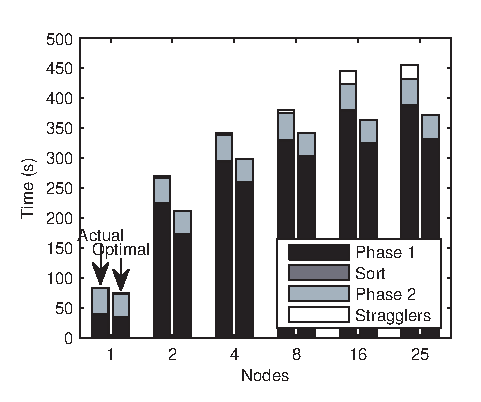
\includegraphics{fig_pds_breakdown2.eps}
\label{fig:pds:sort2:breakdown}
}
\minicaption{With 100~Mbps Ethernet as the bottleneck resource,
  a 100~GB sort benchmark on Parallel DataSeries matches up well with
  the model's prediction and stays within 12-27\% of optimal}
{As more data is sent over the network with larger cluster sizes in
  {\bf (a)}, both the model
  and PDS predict longer sort times that eventually converge.
  A breakdown of time in {\bf (b)} shows that the predicted and actual
  time increases occur during the first map-reduce phase, which
  includes the network data shuffle.}

\label{fig:pds:sort2}
\end{center}
\end{figure}
}

